Otra de las técnicas muestrales muy utilizadas consiste en el denominado muestreo sistemático. Este método consiste en seleccionar aleatoriamente y con la misma probabilidad una unidad entre los primeros ``k'' elementos del marco poblacional. Este entero positivo k se fija previamente y tiene como denominación intervalo muestral. El resto de elementos de la muestra se eligen de una manera sistemática, dejando una separación de k elementos entre todas las unidades seleccionadas. De esta forma, obtenemos las denominadas \textit{muestras 1 en k}.\\

El muestreo sistemático ofrece varias ventajas prácticas, en particular su simplicidad de
ejecución. El hecho de solo realizar una única selección aleatoria es una gran ventaja. Es
fácil, por ejemplo, para un entrevistador seleccionar una muestra sistemática mientras
está en campo.\\

En el muestreo sistemático, podemos decir que existe un efecto que podemos llamar de extensión o ``estratificación'', si cada grupo de k elementos consecutivos a partir del primero se considera como un estrato. No obstante, debe tenerse en cuenta que en el muestreo estratificado la selección se realiza de forma independiente en cada estrato, mientras que en el muestreo sistemático todos los elementos seleccionados ocupan el mismo lugar dentro de cada grupo de k elementos. \\

Entre las ventajas de este tipo de muestreo, se pueden destacar:\\
\begin{itemize}[label=$\bullet$]
    \item Extiende la muestra a toda la población.
    \item Recoge el posible efecto de estratificación debido al orden en que figuran las unidades en la población.
    \item Su aplicación y comprobación son fáciles de realizar.
\end{itemize}

También presenta algunos inconvenientes:\\

\begin{itemize}[label=$\bullet$]
    \item La posibilidad de aumento de la varianza si existe periodicidad.
    \item El problema teórico que se presenta en la estimación de varianzas.
\end{itemize}


\section{Selección de la muestra} \label{sect:5.1}
Como ya se ha comentado anteriormente, la mayor virtud de este muestreo es su simplicidad. Al seleccionar el tamaño de muestra n, se divide la población en n filas, llamadas \textit{zonas sistemáticas} de tamaño $\frac{N}{n} = k$, ordenando a la población en una matriz como la de la figura \ref{fig:sist}, lo cual facilita su comprensión y ejecución.\\

\begin{center}
    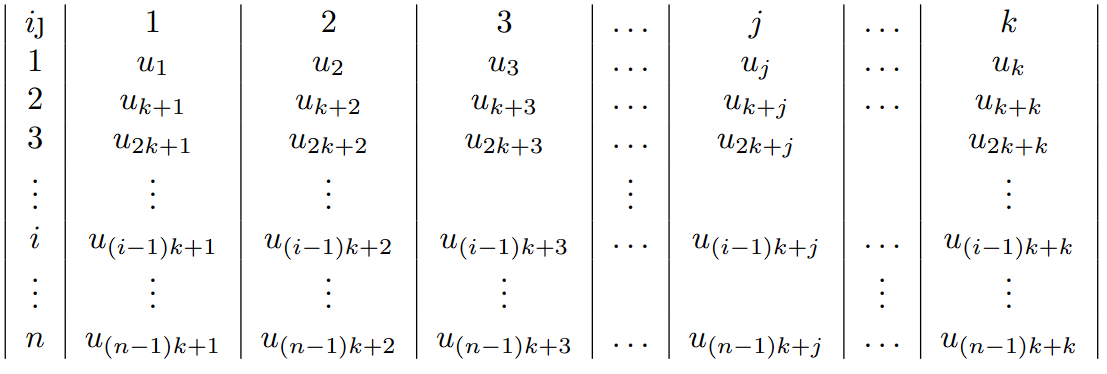
\includegraphics[scale=0.5]{img/sist.png}
    \captionof{figure}{Selección de una muestra sistemática 1 en k.}
    \label{fig:sist}
\end{center}

Una vez ordenada ya solo resta seleccionar un número aleatoriamente  entre 1 y k, el cual determinará la columna del cuadro anterior de la cual obtendremos los elementos de nuestra muestra.\\

En su traducción a un lenguaje informático, el método es muy similar. Los datos serán ordenados como una matriz, pero sin utilizar los objetos \textit{matrix}. Esto se debe a que es posible que no haya un número exacto para formar una matriz con las filas y columnas deseadas por el usuario. Este problema viene dado cuando $\frac{N}{n} = k$ no es un número entero. Para solucionar este problema, k será redondeado hacia abajo y los individuos que no completarían esa última fila de la matriz no serán seleccionados. \\

En algunos casos de la vida real, este problema llega a tener una relevancia importante, como ocurre en el método de selección de miembros a jurado popular. Para obtener estos candidatos, lo que se hace realmente es utilizar un muestreo sistemático con arranque aleatorio. Pero al realizar este tipo de selección, los electores del final de la lista tendrían probabilidad cero de ser elegidos. \\

Para evitar esta deficiencia se publicó el Real Decreto 1398/1995 artículo 3 \cite{RD}, según el cual se mantienen hasta 5 decimales del valor de k, obteniendo por lo tanto una sucesión de índices no exactos. Estos índices serán redondeados para seleccionar los individuos de una muestra que sí abarque toda la población.\\


%%Este problema ya ocurría en la vida real en el problema de selección de miembros del jurado. La solución anterior implica que los individuos situados al final de la lista censal tengan probabilidad nula de ser seleccionados para la muestra. Para evitar esto actualmente y desde la modificación del Real Decreto 1398/1995 artículo 3 \cite{RD} se mantienen hasta 5 decimales del valor de k, obteniendo por lo tanto una sucesión de índices no exactos. Estos índices serán redondeados para seleccionar los individuos de una muestra que sí abarque toda la población.\\%%

Posteriormente elegimos un número al azar entre 1 y k al que denominaremos m, y seleccionaremos los individuos con índice $m+ik, \forall i = 0,...,n-1$. De ésta forma obtenemos los individuos de la columna m siguiendo el ejemplo de la figura \ref{fig:sist}.\\

\section{Análisis de la varianza y correlación} \label{sect:5.2}
En el muestreo sistemático resulta de gran utilidad utilizar una descomposición de la información en un formato análogo al que se utiliza para el análisis de la varianza (Análysis of Variance o ANOVA) ya que nos permite obtener medidas de precisión que nos ayuden a determinar el método de estimación más preciso para nuestros datos de entre los posibles. \\

La tabla ANOVA poblacional para el análisis sistemático contiene los siguientes valores:\\

\begin{table}[H]
\centering

\begin{tabular}{|c|c|c|c|}
\hline
Fuente de variación & \begin{tabular}[c]{@{}c@{}}Grados de\\  libertad\end{tabular} & \begin{tabular}[c]{@{}c@{}}Sumas de\\ cuadrados\end{tabular}  & \begin{tabular}[c]{@{}c@{}}Cuadrados\\  medios\end{tabular} \\ \hline
Entre muestras   & $k-1$   & $\sum\limits_{i}^n\sum\limits_{j}^k(\bar{x}_j-\bar{X})^2$ & $S_{bs}^2$       \\ \hline
Intramuestras    & $N-k$   & $\sum\limits_{i}^n\sum\limits_{j}^k(X_{ij}-\bar{x}_j)^2$  & $S_{ws}^2$       \\ \hline
Total            & $N-1$   & $\sum\limits_{i}^n\sum\limits_{j}^k(X_{ij}-\bar{X})$      & $S^2$   \\ \hline        
\end{tabular}
\caption{Tabla ANOVA}
\label{tab:anova}
\end{table}

Donde $S_{bs}^2$ es la cuasivarianza intermuestral definida por:\\
\begin{equation}
    \frac{\sum\limits_{i}^n\sum\limits_{j}^k(\bar{x}_j-\bar{X})^2}{k-1}
\end{equation}

Y $S_{ws}^2$ la cuasivarianza intramuestral:\\

\begin{equation}
    \frac{\sum\limits_{i}^n\sum\limits_{j}^k(X_{ij}-\bar{x}_j)^2}{N-k}
\end{equation}

Pudiendo escribir la siguiente igualdad:\\

\begin{equation}
    (N-1)S^2 = (N-k)S_{bs}^2 + (k-1)S_{ws}^2
\end{equation}

La comparación de la cuasivarianza intermuestral e intramuestral con la cuasivarianza poblacional nos permite realizar una comparación de los distintos tipos de muestreo vistos hasta ahora. \\

Si $S_{bs}^2 > S^2$ entonces el muestreo sistemático será más preciso que el muestreo estratificado. De la misma forma si $S_{ws}^2 > S^2$ el muestreo sistemático será más preciso que el aleatorio simple. A igualdad de cuasivarianzas la precisión será la misma en ambos tipos de muestreo.\\

Otras medidas de comparación son los coeficientes de correlación intramuestral e intermuestral. Se define el primero como:\\

\begin{equation}
    \rho_{w} = \frac{2\sum\limits_j^k\sum\limits_{i<z}^n(X_{ij}-\bar{X})(X_{zj}-\bar{X})}{N(n-1)\sigma^2}
\end{equation}

 que obtiene la precisión mínima con valor 1 y precisión máxima con valor $\frac{-1}{n-1}$.\\
 
 Con $\rho_w = 0$ la precisión del muestreo sistemático coincide con el aleatorio simple con reposición. Entre este valor y 1 el muestreo aleatorio simple será más preciso que el sistemático. Valores menores que 0 hasta el valor de varianza mínima suponen el caso contrario.\\

 El coeficiente de correlación intermuestral viene dado por la expresión:
 
\begin{equation}
    \rho_{wst} = \frac{2\sum\limits_j^k\sum\limits_{i<z}^n(X_{ij}-\bar{X_i})(X_{zj}-\bar{X_z})}{n(n-1)(k-1)S_{wst}^2}
\end{equation}

 que obtiene sus valores de precisión mínima y máxima de la misma forma que con la correlación intramuestral y con la misma interpretación de sus valores permite comparar la precisión entre el muestreo sistemático y el muestreo estratificado.


\section{Estimadores lineales insesgados} \label{sect:5.3}

Sustituyendo en la fórmula general para una muestra sistemática, obtenemos los estimadores lineales insesgados en el muestreo sistemático:

\begin{equation}
    \hat{\theta} = \hat{X} = \sum_{i=1}^{n}\sum_{j=1}^1\frac{X_{ij}}{\frac{1}{k}} = \sum_{i=1}^{n}kX_{ij} = N\frac{1}{n}\sum_{i=1}^{n}X_{ij} = N\bar{x_j}
\end{equation}

\begin{equation}
    \hat{\theta} = \hat{\bar{X}} = \sum_{i=1}^{n}\sum_{j=1}^1\frac{\frac{X_{ij}}{N}}{\frac{1}{k}} = \frac{1}{n}\sum_{i=1}^{n}X_{ij} = \bar{x_j}
\end{equation}

\begin{equation}
    \hat{\theta} = \hat{P} =  \sum_{i=1}^{n}\sum_{j=1}^1\frac{\frac{A_{ij}}{N}}{\frac{1}{k}} = \frac{1}{n}\sum_{i=1}^{n}A_{ij} = \bar{P_j}
\end{equation}

\begin{equation}
    \hat{\theta} = \hat{A}  = \sum_{i=1}^{n}\sum_{j=1}^1\frac{A_{ij}}{\frac{1}{k}} = N\frac{1}{n}\sum_{i=1}^{n}A_{ij} = N\bar{P_j}
\end{equation}

\section{Estimadores de la varianza} \label{sect:5.4}
La estimación de la varianza es uno de los mayores problemas del muestreo sistemático. Al no tener un método directo, disponemos de 3 métodos de estimación diferentes con distintos resultados. En el apartado \ref{sect:6.2} vimos cómo, a partir de los valores de cuasivarianzas y correlaciones, se puede saber qué tipo de muestreo es más preciso.
Diferenciamos 3 casos:\\

\textbf{$\bullet$ \boldmath$\rho_w$ próximo a 0}\\

En el caso de $\rho_w$ positivo y próximo a 0 podemos suponer que la población está ordenada de forma aleatoria, por lo que podremos estimar la varianza con las fórmulas de muestreo aleatorio simple sobre nuestra muestra sistemática.\\

\textbf{$\bullet$ \boldmath$\rho_{wst}$ próximo a 0}\\

Para valores positivos próximos a 0 de $\rho_{wst}$ se puede considerar la falta de aleatoriedad en la selección de la muestra sobre cada zona sistemática (fila) de nuestra matriz de población. Por ello la varianza se estima tomando cada fila como un estrato y realizando las estimaciones sobre una muestra estratificada con una unidad por estrato.\\

En la práctica se supone un estrato cada 2 zonas sistemáticas, teniendo en la muestra $\frac{n}{2}$ estratos de 2 individuos por estrato. En los casos en los que $\frac{n}{2}$ no sea un número entero se repite un individuo al azar de la muestra al final para cuadrar los resultados.\\

\textbf{$\bullet$ Ni \boldmath$\rho_w$ ni \boldmath$\rho_{wst}$ próximos a 0}\\

En este caso utilizaremos el método de las muestras interpenetrantes, que se utiliza para formar un estimador cuando tenemos una o más muestras elegidas con el mismo esquema de muestreo y proporcionen por sí mismas un estimador válido del parámetro con el mismo error de muestreo.\\

Para ello se indica un parámetro extra t que representa el número de arranques o submuestras que utilizaremos para la estimación. En lugar de tomar la muestra tomada originalmente de tamaño n tomaremos t submuestras sistemáticas de tamaño $\frac{n}{t}$.\\

A partir de las submuestras podemos formar estimadores de la media y el total como:

\begin{equation}
    \bar{x_c} = \frac{1}{t}\sum_1^t\bar{x_i}
\end{equation}

\begin{equation}
    x_c = \frac{1}{t}N\sum_1^t\bar{x_i}
\end{equation}

Y sus estimadores de varianzas:

\begin{equation}
    \widehat{V(\bar{x_c})} = \frac{1}{t(1-t)}\sum_1^t(\bar{x_i}^2-\bar{x_c}^2)
\end{equation}

\begin{equation}
    \widehat{V(x_c)} = \frac{1}{t(1-t)}\sum_1^t((N\bar{x_i})^2-x_c^2)
\end{equation}

\section{Aplicaciones para el muestreo sistemático de la librería samplingR}

Las funciones desarrolladas para la aplicación de los conceptos teóricos mostrados en este capítulo utilizarán el prefijo \textit{syst} como abreviación de \textit{systematic sampling}, y son las siguientes.

\begin{itemize}[label=$\bullet$]
    \item syst.sample: Dado un tamaño poblacional N y un tamaño de muestra n devuelve una muestra sistemática, comunmente denominada 1 en k. En caso de aportar un conjunto de datos devolverá los individuos de los datos que conforman la muestra. Al ser esto opcional, si no se aporta un conjunto de datos devolverá los índices de los individuos que conforman la muestra.\\

    Realiza las funciones explicadas en el apartado \ref{sect:5.1}.

    \item syst.all.samples: Función que devuelve todas las posibles muestras sistemáticas dato un tamaño de muestra n y un tamaño poblacional N.

    \item syst.anova: Obtiene una tabla de análisis de la varianza sobre los datos de la población, siguiendo el esquema comentado en la tabla \ref{tab:anova}.

    \item syst.intercorr: Realiza el cálculo del coeficiente de correlación interclase de los datos. 

    \item syst.intracorr: Realiza el cálculo del coeficiente de correlación intraclase de los datos. \\
    
    Esto permite realizar una comparación de la precisión de la estimación entre el muestreo sistemático y el muestreo aleatorio simple.\\

     Estas tres funciones abarcan los conceptos explicados en el apartado \ref{sect:5.2}.

    \item syst.estimator: Dada una muestra de datos obtiene el estimador poblacional del parámetro especificado. También calcula su varianza estimada, error de muestreo y opcionalmente su error de estimación y un intervalo de confianza si se especifica el coeficiente de confianza en el parámetro \textit{alpha}. \\

    Realiza las funciones explicadas en el apartado \ref{sect:5.3} y \ref{sect:5.4}.

    

\end{itemize}